\documentclass{article}
%-----------------------------------------------------------------------------------------------------------------------------------------------------------------------------
% Packages
\usepackage[margin=1in,includefoot]{geometry}
\usepackage{enumitem}
\usepackage{caption}
\usepackage{titlesec}
\usepackage{amsmath}
\usepackage{empheq}
\usepackage{imakeidx}
\usepackage[utf8]{inputenc}
\usepackage{color}
\usepackage[acronym,style=tree]{glossaries}
\usepackage[automake]{glossaries-extra}
\usepackage{graphicx}
%-----------------------------------------------------------------------------------------------------------------------------------------------------------------------------
\graphicspath{{./Images/}}
%-----------------------------------------------------------------------------------------------------------------------------------------------------------------------------
% Sets automatic numbering system in \paragraph
\setcounter{secnumdepth}{4}
\titleformat{\paragraph}
{\normalfont\normalsize\bfseries}{\theparagraph}{1em}{}
\titlespacing*{\paragraph}
{0pt}{3.25ex plus 1ex minus .2ex}{1.5ex plus .2ex}
%-----------------------------------------------------------------------------------------------------------------------------------------------------------------------------
% Custom Box for Mathematical Formulae
\definecolor{myblue}{rgb}{.8, .8, 1}
\newlength\mytemplen
\newsavebox\mytempbox
\makeatletter
\newcommand\mybluebox{%
    \@ifnextchar[%]
       {\@mybluebox}%
       {\@mybluebox[0pt]}}
\def\@mybluebox[#1]{%
    \@ifnextchar[%]
       {\@@mybluebox[#1]}%
       {\@@mybluebox[#1][0pt]}}
\def\@@mybluebox[#1][#2]#3{
    \sbox\mytempbox{#3}%
    \mytemplen\ht\mytempbox
    \advance\mytemplen #1\relax
    \ht\mytempbox\mytemplen
    \mytemplen\dp\mytempbox
    \advance\mytemplen #2\relax
    \dp\mytempbox\mytemplen
    \colorbox{myblue}{\hspace{1em}\usebox{\mytempbox}\hspace{1em}}}
\makeatother
%-----------------------------------------------------------------------------------------------------------------------------------------------------------------------------
% Allows for the creation of the glossary
\makeglossaries
%-----------------------------------------------------------------------------------------------------------------------------------------------------------------------------
% Glossary Terms

% -- Acceptor Concentration
\newglossaryentry{Acceptor Concentration}
{
	name=Acceptror Concentration,
	description={The concentration of holes (absense of electrons) free to accept electrons within a specific volume \cite{OneOneNeamen}}
}

% -- Bandgap Energy
\newglossaryentry{Bandgap Energy}
{
	name=Bandgap Energy,
	description={The minimal amount of energy if takes for an electron to break the covalent bond and become a valence electron \cite{OneOneNeamen}}
}

% -- Boltzmann's Constant
\newglossaryentry{Boltzmann's Constant} 
{
	name=Boltzmann's Constant,
	description={Physical constant relating the average kinetic energy of particles in a gas \cite{boltzmannsConstant}}
}

% -- Built in Potential Barrier
\newglossaryentry{Built-in Potential Barrier}
{
	name=Buit-in Potential Barrier,
	description={The potential difference (voltage) across a pn junction \cite{OneTwoNeamen}}
}

% -- Charge of an Electron (e)
\newglossaryentry{Charge of an Electron}
{
	name=Charge of an Electron,
	description={Electronic charge of a single electron \cite{OneOneNeamen}}
}

% -- Common-Base Current Gain
\newglossaryentry{Common-Base Current Gain}
{
	name=Common-Base Current Gain,
	description={A constant which describes the relationship between the collector and emitter currents in a transistor as a ratio between the two respectively. The collector current is a factor or magnitude smaller than the emitter current, which is represented by this constant. This constant should never be lower or equal to 1 in a valid and operating transistor \cite{FiveOneNeamen}}
}

% -- Common-Emitter Current Gain
\newglossaryentry{Common-Emitter Current Gain}
{
	name=Common-Emitter Current Gain,
	description={A constant which describes the relationship between the collector and base currents in a transistor as a ratio between the two respectively. The collector current is a factor or magnitude larger than the base current, which is represented by this constant. This constant should never be lower or equal to 1 in a valid and operating transistor \cite{FiveOneNeamen}}
}

% -- Compound Semiconductor
\newglossaryentry{Compound Semiconductor}
{
	name=Compound Semiconductor,
	description={A semiconductor composed of elements from group III and V of the Periodic Table of Elements \cite{OneOneNeamen}}
}

% -- Conductance
\newglossaryentry{Conductance}
{
	name=Conductance,
	description={A measure of a material's ability to conduct an electric current \cite{conductivityResistivity}}
}

% -- Covalent Bond
\newglossaryentry{Covalent Bond}
{
	name=Covalent Bond,
	description={Bonds formed by the sharing of valence electrons between atoms \cite{OneOneNeamen}}
}

% -- Cutoff
\newglossaryentry{Cutoff}
{
	name=Cutoff,
	description={When the base-emitter voltage of a transistor has zero applied volts \cite{FiveOneNeamen}}
}

% -- Current Density of Electrons
\newglossaryentry{Current Density of Electrons}
{
	name=Current Density of Electrons,
	description={The current due to the flow of the electrons within a specified volume \cite{OneOneNeamen}}
}

% -- Current Density of Holes
\newglossaryentry{Current Density of Holes}
{
	name=Current Density of Holes,
	description={The current due to the flow of holes within a specified volume  \cite{OneOneNeamen}}
}

% -- -- Diffusion Current Density of Electrons
\newglossaryentry{Diffusion Current Density of Electrons}
{
	name=Diffusion Current Density of Electrons,
	description={The current due to the flow of electrons within a specified volume due to the process of diffusion \cite{OneOneNeamen}},
	parent=Current Density of Electrons
}

% -- -- Diffusion Current Density of Holes
\newglossaryentry{Diffusion Current Density of Holes}
{
	name=Diffusion Current Density of Holes,
	description={The current due to the flow of holes within a specified volume due to the process of diffusion \cite{OneOneNeamen}},
	parent=Current Density of Holes
}

% -- Donor Concentration
\newglossaryentry{Donor Concentration}
{
	name=Donor Concentration,
	description={The concentration of electrons free to donate in a material \cite{OneOneNeamen}}
}

% -- Donor Impurity
\newglossaryentry{Donor Impurity}
{
	name=Donor Impurity,
	description={A material, that when added to the composition of a semiconductor, allows for the controlled creation of free electrons without the creation of holes within the material \cite{OneTwoNeamen}}
}

% -- -- Drift Currrent Density of Electrons
\newglossaryentry{Drift Current Density of Electrons}
{
	name=Drift Current Density of Electrons,
	description={The current due to the flow electrons within a specified volume due to the pull of an electric field \cite{OneOneNeamen}},
	parent=Current Density of Electrons
}

% -- -- Drift Current Density of Holes
\newglossaryentry{Drift Current Density of Holes}
{
	name=Drift Current Density of Holes, 
	description={The current due to the flow of holes within a specified volume due to the pull of an electric field \cite{OneOneNeamen}},
	parent=Current Density of Holes
}

% -- Drift Velocity of Electrons
\newglossaryentry{Drift Velocity of Electrons}
{
	name=Drift Velocity of Electrons,
	description={The average speed of electrons \cite{OneOneNeamen}}
}

% -- Drift Velocity of Holes
\newglossaryentry{Drift Velocity of Holes}
{
	name=Drift Velocity of Holes,
	description={The average speed of holes \cite{OneOneNeamen}}
}

% -- Electric Field
\newglossaryentry{Electric Field}
{
	name=Electric Field,
	description={The electric field applied \cite{OneOneNeamen}}
}

% -- Electron Mobility
\newglossaryentry{Electron Mobility}
{
	name=Electron Mobility,
	description={How well an electron is able to move in a semiconductor \cite{OneOneNeamen}}
}

% -- Elemental Semiconductor
\newglossaryentry{Elemental Semiconductor}
{
	name=Elemental Semiconductor,
	description={A semiconductor composed of elements from group IV of the Periodic Table of Elements \cite{OneOneNeamen}}
}

% -- Free Electrons
\newglossaryentry{Free Electrons}
{
	name=Free Electrons,
	description={The concentration of electrons within a material which are not bound to an atom. Is measured in the number of electrons per volume cubed \cite{OneOneNeamen}}
}

% -- Forbidden Bandgap
\newglossaryentry{Forbidden Bandgap}
{
	name=Forbidden Bandgap,
	description={The phenomenon that an electron may not have any amount of energy less than that of the valance band, and more than that of the conductance band. The amount of energy required to move an electron from the conductance band to the valence band is the bandgap energy \cite{OneOneNeamen}}
}

% -- Free Holes
\newglossaryentry{Free Holes}
{
	name=Free Holes,
	description={The concentration of atoms within a material which has a hole in which an electron may enter. Is measured in the number of holes per volume cubed \cite{OneOneNeamen}}
}

% -- Hole
\newglossaryentry{Hole}
{
	name=Hole,
	description={An atom which has space availiable in the valence band for a free electron, denoted as a positive particle \cite{OneOneNeamen}}
}

% -- Hole Mobility
\newglossaryentry{Hole Mobility}
{
	name=Hole Mobility,
	description={How well a hole (area of the absence of electrons) is able to move in a semiconductor \cite{OneOneNeamen}}
}

% -- Insulator
\newglossaryentry{Insulator}
{
	name=Insulator,
	description={A material in which current cannot flow because the electrons are bound in their respective atoms with a certain amount of resistance \cite{OneOneNeamen}}
}

% -- Intrinsic Carrier Concentration
\newglossaryentry{Intrinsic Carrier Concentration}
{
	name=Intrinsic Carrier Concentration,
	description={The concentration of free electrons and holes within a specified volume \cite{OneOneNeamen}}
}

% -- Intrinsic Semiconductor
\newglossaryentry{Intrinsic Semiconductor}
{
	name=Intrinsic Semiconductor,
	description={A single-crystal semiconductor material composed of a single element from the Periodic Table of Elements \cite{OneOneNeamen}}
}

% -- Junction Capacitance
\newglossaryentry{Junction Capacitance}
{
	name=Junction Capacitance,
	description={Capacitance across a pn junction \cite{OneTwoNeamen}}
}

% -- Metallurgical Junction
\newglossaryentry{Metallurgical Junction}
{
	name=Metallurgical Junction,
	description={Junction in which an n and p type material are connected. Located at x=0 \cite{OneTwoNeamen}}
}

% -- Recombination
\newglossaryentry{Recombination}
{
	name=Recombination,
	description={The process of free electrons and holes attracting and combining together \cite{OneOneNeamen}}
}

% -- Reverse-Bias Saturation Current
\newglossaryentry{Reverse-Bias Saturation Current}
{
	name=Reverse-Bias Saturation Current,
	description={Current which flows from donor to acceptor in a pn junction when there is no voltage applied across the junction \cite{OneTwoNeamen}}
}

% -- Resistivity
\newglossaryentry{Resistivity}
{
	name=Resistivity,
	description={A measure of how strongly a given material opposes sthe flow of electric current \cite{conductivityResistivity}}
}

% -- Semiconductor Material Constant
\newglossaryentry{Semiconductor Material Coefficient}
{
	name=Semiconductor Material Coefficient,
	description={Semiconductor material coefficient constant \cite{OneOneNeamen}}
}

% -- Temperature
\newglossaryentry{Temperature}
{
	name=Temperature,
	description={The temperature of an object or space \cite{OneOneNeamen}}
}

% -- Thermal Voltage
\newglossaryentry{Thermal Voltage}
{
	name=Thermal Voltage,
	description={The built-in voltage of a semiconductor at room temperature (T=300K) \cite{OneTwoNeamen}}
}

% -- Total Drift Velocity
\newglossaryentry{Total Drift Current Density}
{
	name=Total Drift Current Density,
	description={The sum of the hole and electron current within a specified volume due to the pull of an electric field \cite{OneOneNeamen}}
}

% -- Valence Electrons
\newglossaryentry{Valence Electrons}
{
	name=Valence Electrons,
	description={Electrons in the outermost shell of an atom. May be passed on to another atom and form a covalent bond, and is therefore also deemed a \textit{free electron} \cite{OneOneNeamen}}
}
%-----------------------------------------------------------------------------------------------------------------------------------------------------------------------------
% Variables
\newacronym{$N_a$}{$N_a$}{Acceptor Concentration}
\newacronym{$E_g$}{$E_g$}{Bandgap Energy}
\newacronym{$k$}{$k$}{Boltzmann's Constant $(86x10^{-6} \frac{eV}{k})$}
\newacronym{$V_{bi}$}{$V_{bi}$}{Built-in Potential Barrier}
\newacronym{$e$}{$e$}{Charge of an Electron $(1.6x10^{19})$}
\newacronym{Common Base Current Gain}{$\alpha$}{Collector Base Current Gain}
\newacronym{Common Emitter Current Gain}{$\beta$}{Collector Emitter Current Gain}
\newacronym{$n$}{$n$}{Concentration of Electrons}
\newacronym{$p$}{$p$}{Concentration of Holes}
\newacronym{Conductance of a Semiconductor}{$\sigma$}{Conductance}
\newacronym{$i_D$}{$i_D$}{Current Through a pn Junction (Diode)}
\newacronym{$Jn$}{$Jn$}{Diffusion Current Density of Electrons}
\newacronym{$Jp$}{$Jp$}{Diffusion Current Density of Holes}
\newacronym{$x$}{$x$}{Distance}
\newacronym{$N_d$}{$N_d$}{Donor Concentration}
\newacronym{$J_n$}{$J_n$}{Drift Current Density of Electrons}
\newacronym{$J_p$}{$J_p$}{Drift Current Density of Holes}
\newacronym{$v_{dn}$}{$v_{dn}$}{Drift Velocity of Electrons}
\newacronym{$v_{dp}$}{$v_{dp}$}{Drift Velocity of Holes}
\newacronym{$E$}{$E$}{Electric Field Applied}
\newacronym{$D_n$}{$D_n$}{Electron Diffusion Coefficient}
\newacronym{$v_D$}{$v_D$}{Forward-Bias Voltage}
\newacronym{$n_o$}{$n_o$}{Free Electrons}
\newacronym{$p_o$}{$p_o$}{Free Holes}
\newacronym{$D_p$}{$D_p$}{Hole Diffusion Coefficient}
\newacronym{$n_i$}{$n_i$}{Intrinsic Carrier Concentration}
\newacronym{$C_j$}{$C_j$}{Juncton Capacitance}
\newacronym{$C_{jo}$}{$C_{jo}$}{Junction Capacitance at Zero Applied Voltage}
\newacronym{Mobility of a Hole}{$\mu_p$}{Mobility of a Hole}
\newacronym{Mobility of an Electron}{$\mu_n$}{Mobility of an Electron}
\newacronym{Recombination Factor}{$\delta$}{Electron-Hole Recombination Factor}
\newacronym{Resistivity of a Semiconductor}{$\rho$}{Resistivity}
\newacronym{$V_R$}{$V_R$}{Reverse-Biased Voltage}
\newacronym{$I_S$}{$I_S$}{Reverse-Bias Saturation Current (DC Conditions)}
\newacronym{$i_S$}{$i_S$}{Reverse-Bias Saturation Current (AC Conditions)}
\newacronym{$B$}{$B$}{Semiconductor Material Constant}
\newacronym{$T$}{$T$}{Temperature}
\newacronym{$V_T$}{$V_T$}{Thermal Voltage}
\newacronym{$J$}{$J$}{Total Drift Current Density}
\newacronym{$i_B$}{$i_B$}{Base Current (AC Conditions)}
\newacronym{$i_C$}{$i_C$}{Collector Current (AC Conditions)}
\newacronym{$i_E$}{$i_E$}{Emitter Current (AC Conditions)}
\newacronym{$I_B$}{$I_B$}{Base Current (DC Conditions)}
\newacronym{$I_C$}{$I_C$}{Collector Current (DC Conditions)}
\newacronym{$I_E$}{$I_E$}{Emitter Current (DC Conditions)}
%-----------------------------------------------------------------------------------------------------------------------------------------------------------------------------
% Index Stuff
\makeindex[columns=1]
%-----------------------------------------------------------------------------------------------------------------------------------------------------------------------------
\begin{document}
\pagenumbering{gobble}
%-----------------------------------------------------------------------------------------------------------------------------------------------------------------------------
% Title Page
\title{Semiconductor, Diode, and Transistor Reference}
\author{Angelino Lefevers}
\maketitle
\thispagestyle{empty}
\cleardoublepage
%-----------------------------------------------------------------------------------------------------------------------------------------------------------------------------
% Table of Contents
\tableofcontents
\thispagestyle{empty}
\cleardoublepage
%-----------------------------------------------------------------------------------------------------------------------------------------------------------------------------
% Introduction
\section*{Introduction}
\addcontentsline{toc}{section}{Introduction}
Just throwing together some concepts and examples for later reference
\cleardoublepage
%-----------------------------------------------------------------------------------------------------------------------------------------------------------------------------
% --- --- --- --- --- --- --- ---  Semiconductor Physics, Materials, and Properties --- --- --- --- --- --- --- --- 
\section{Semiconductor Physics, Materials, and Properties}
\pagenumbering{arabic}
\setcounter{page}{1}
%-----------------------------------------------------------------------------------------------------------------------------------------------------------------------------
% Semiconductor Properties and Constants
\subsection{Semiconductor Properties and Constants}

% Common Semiconductor Constants
\subsubsection{Common Semiconductor Constants}
\begin{center}
\captionof{table}{Semiconductor Constants}
\begin{tabular}{|l|l|l|}
\hline
Material & Eg(eV) & B(cm\textsuperscript{-3}K\textsuperscript{-3/2}) \\
\hline
Silicon (Si) & 1.1 & 5.23x10\textsuperscript{15} \\
Gallium Arsenide (GaAs) & 1.4 & 2.10x10\textsuperscript{14} \\
Germanium (Ge) & 0.66 & 1.66x10\textsuperscript{15} \\
\hline
\end{tabular}
\end{center}

% Boltzmann's Constant
\subsubsection{Boltzmann's Constant}
\begin{empheq}[box={\mybluebox[5pt]}]{equation*}
k = 86x10^{-6}\frac{eV}{k}
\end{empheq}
\index{Boltzmann's Constant}

% Einstein's Relation
\subsubsection{Einstein's Relation}

\begin{empheq}[box={\mybluebox[5pt]}]{equation*}
\frac{D_n}{\mu_n} = \frac{D_p}{\mu_p} = \frac{kT}{e} \cong 0.026 V
\end{empheq}

\begin{itemize}
\item e :=Charge of an Electron $(1.6x10^{-19} eV)$ \index{Charge of an Electron}
\item T := Temperature (K) \index{Temperature}
\item k := Boltzmann's Constant $(86x10^{-6}) (\frac{eV}{k})$ \index{Boltzmann's Constant}
\item $\mu_n$  := Electron Mobility $(\frac{cm^2}{V-s})$ \index{Electron Mobility}
\item $\mu_n$ := Hole Mobility $(\frac{cm^2}{V-s})$ \index{Hole Mobility}
\item $D_n$ := Electron Diffusion Coefficient $(\frac{cm^2}{s})$ \index{Electron Diffusion Coefficient}
\item $D_p$ := Hole Diffusion Coefficient $(\frac{cm^2}{s})$ \index{Hole Diffusion Coefficient}
\end{itemize}

% Conducance
\subsubsection{Conductance}
\begin{empheq}[box={\mybluebox[5pt]}]{equation*}
\sigma = en\mu_n + ep\mu_p
\end{empheq}

\begin{itemize}
\item e :=Charge of an Electron $(1.6x10^{-19} eV)$ \index{Charge of an Electron}
\item $\sigma$ := Conductance $((\Omega-cm)^{-1})$ \index{Conductance}
\item $\mu_n$  := Electron Mobility $(\frac{cm^2}{V-s})$ \index{Electron Mobility}
\item $\mu_n$ := Hole Mobility $(\frac{cm^2}{V-s})$ \index{Hole Mobility}
\end{itemize} 

% Resistivity
\subsubsection{Resistivity}
\begin{empheq}[box={\mybluebox[5pt]}]{equation*}
\rho = \frac{1}{\sigma}
\end{empheq}

\begin{itemize}
\item $\sigma$ := Conductance $((\Omega-cm)^{-1})$ \index{Conductance}
\item $\rho$ := Resistivity $(\Omega-cm)$ \index{Resistivity}
\end{itemize}

% Intrinsic Carrier Concentration
\subsubsection{Intrinsic Carrier Concentration}
Returns the concentration of free electrons and holes in a material.
\begin{empheq}[box={\mybluebox[5pt]}]{equation*}
n_i = BT^{3/2}e^{-(E_g/2kT)}
\end{empheq}
\begin{itemize}
\item \acrshort{$B$} := Semiconductor Material Coefficient $(cm^{-3}K^{-3/2})$ \index{Semiconductor Material Coefficient}
\item T := Temperature (K) \index{Temperature}
\item k := Boltzmann's Constant $(86x10^{-6}) (\frac{eV}{k})$ \index{Boltzmann's Constant}
\item $E_g$ := Bandgap Energy (eV) \index{Bandgap Energy}
\item $n_i$ := Intrinsic Carrier Concentration $(\frac{\# of electrons}{cm^3})$ \index{Intrinsic Carrier Concentration}
\end{itemize}

% Fundamental Relationship Between Electron and Hole Concentration
\subsubsection{Fundamental Relationship Between Electron and Hole Concentration}
\begin{empheq}[box={\mybluebox[5pt]}]{equation*}
n_{o}p_{o} = n_i^2
\end{empheq}

\begin{itemize}
\item $n_i$ := Intrinsic Carrier Concentration $(\frac{\# of electrons}{cm^3})$ \index{Intrinsic Carrier Concentration}
\item $n_o$ := Concentration of Free Electrons at Thermal Equalibrium $(\frac{\# of electrons}{cm^3})$ \index{Free Electrons}
\item $p_o$ := Concentration of Free Holes at Thermal Equalibrium $(\frac{\# of holes}{cm^3})$ \index{Free Holes}
\end{itemize}

% -- n - type
\paragraph{n-type}

\begin{empheq}[box={\mybluebox[5pt]}]{equation*}
n_o \cong N_d
\end{empheq}

\begin{empheq}[box={\mybluebox[5pt]}]{equation*}
p_o = \frac{n_i^2}{N_d}
\end{empheq}

\begin{itemize}
\item $N_d$ := Donor Concentration (cm\textsuperscript{-3}) \index{Donor Concentration}
\end{itemize}

% -- p - type
\paragraph{p-type}

\begin{empheq}[box={\mybluebox[5pt]}]{equation*}
p_o \cong N_a
\end{empheq}

\begin{empheq}[box={\mybluebox[5pt]}]{equation*}
n_o = \frac{n_i^2}{N_a}
\end{empheq}

\begin{itemize}
\item $N_a$ := Acceptor Concentration (cm\textsuperscript{-3})  \index{Acceptor Concentration}
\end{itemize}

% Excess Carriers
\subsubsection{Excess Carriers}
\begin{empheq}[box={\mybluebox[5pt]}]{equation*}
n = n_o + n\delta
\end{empheq}

\begin{empheq}[box={\mybluebox[5pt]}]{equation*}
p = p_o + p\delta
\end{empheq}

\begin{itemize}
\item n := Electron Concentration $(\frac{\# of electrons}{cm^3})$
\item p := Hole Concentration $(\frac{\# of holes}{cm^3})$
\item $n_o$ := Concentration of Free Electrons at Thermal Equalibrium $(\frac{\# of electrons}{cm^3})$ \index{Free Electrons}
\item $p_o$ := Concentration of Free Holes at Thermal Equalibrium $(\frac{\# of holes}{cm^3})$ \index{Free Holes}
\item $\delta$ := Recombination Factor \index{Recombination}
\end{itemize}

\cleardoublepage
%-----------------------------------------------------------------------------------------------------------------------------------------------------------------------------
% Current in Semiconductors
\subsection{Current in Semiconductors}

% Drift Velocity
\subsubsection{Drift Velocity}

\begin{empheq}[box={\mybluebox[5pt]}]{equation*}
v_{dn} = -\mu_{n}E
\end{empheq}

\begin{empheq}[box={\mybluebox[5pt]}]{equation*}
v_{dp} = \mu_{p}E
\end{empheq}

\begin{itemize}
\item E := Electric Field $(\frac{V}{cm})$ \index{Electric Field}
\item $\mu_n$  := Electron Mobility $(\frac{cm^2}{V-s})$ \index{Electron Mobility}
\item $\mu_n$ := Hole Mobility $(\frac{cm^2}{V-s})$ \index{Hole Mobility}
\item $v_{dn}$ := Drift Velocity of Electrons $(\frac{cm}{s})$ \index{Drift Velocity of Electrons}
\item $v_{dp}$ := Drift Velocity of Holes $(\frac{cm}{s})$ \index{Drift Velocity of Holes}
\end{itemize}

\cleardoublepage

% Drift Current Velocity
\subsubsection{Drift Current Density}

\begin{empheq}[box={\mybluebox[5pt]}]{equation*}
J_n = -env_{dn} = -en(-\mu_{n}E) = en\mu_{n}E
\end{empheq}

\begin{empheq}[box={\mybluebox[5pt]}]{equation*}
J_p = epv_{dp} = ep(\mu_{p}E) = ep\mu_{p}E
\end{empheq}

\begin{empheq}[box={\mybluebox[5pt]}]{equation*}
J = en\mu_{n}E + ep\mu_{p}E = E\sigma = \frac{1}{\rho}E
\end{empheq}

\begin{itemize}
\item e :=Charge of an Electron $(1.6x10^{-19} eV)$ \index{Charge of an Electron}
\item E := Electric Field $(\frac{V}{cm})$ \index{Electric Field}
\item $\sigma$ := Conductance $((\Omega-cm)^{-1})$ \index{Conductance}
\item $\rho$ := Resistivity $(\Omega-cm)$ \index{Resistivity}
\item n := Electron Concentration $(\frac{\# of electrons}{cm^3})$
\item p := Hole Concentration $(\frac{\# of holes}{cm^3})$
	\begin{itemize}
	\item n-type := \begin{empheq}[box={\mybluebox[5pt]}]{equation*}n = N_d\end{empheq} \\
			    \begin{empheq}[box={\mybluebox[5pt]}]{equation*}p = \frac{n_i^2}{N_d}\end{empheq}
	\item p-type := \begin{empheq}[box={\mybluebox[5pt]}]{equation*}p = N_a\end{empheq} \\
			    \begin{empheq}[box={\mybluebox[5pt]}]{equation*}n = \frac{n_i^2}{N_a}\end{empheq}
	\end{itemize}
\item $\mu_n$  := Electron Mobility $(\frac{cm^2}{V-s})$ \index{Electron Mobility}
\item $\mu_n$ := Hole Mobility $(\frac{cm^2}{V-s})$ \index{Hole Mobility}
\item $v_{dn}$ := Drift Velocity of Electrons $(\frac{cm}{s})$ \index{Drift Velocity of Electrons}
\item $v_{dp}$ := Drift Velocity of Holes $(\frac{cm}{s})$ \index{Drift Velocity of Holes}
\item $J_n$ := Drift Current Density of Electrons $(\frac{A}{cm^2})$ \index{Drift Current Density of Electrons}
\item $J_p$ := Drift Current Density of Holes $(\frac{A}{cm^2})$ \index{Drift Current Density of Holes}
\item J := Total Drift Current Density in a Semiconductor $(\frac{A}{cm^2})$ \index{Total Drift Current Density}
\end{itemize}

% Diffusion Current Density
\subsubsection{Diffusion Current Density}

% -- Diffusion Current Density due to the Flow of Electrons
\paragraph{Diffusion Current Density due to the Flow of Electrons}
\begin{empheq}[box={\mybluebox[5pt]}]{equation*}
Jn = eD_n\frac{dn}{dx}
\end{empheq}

% -- Diffusion Current Density due to the Flow of Holes
\paragraph{Diffusion Current Density due to the Flow of Holes}
\begin{empheq}[box={\mybluebox[5pt]}]{equation*}
Jp = -eD_p\frac{dp}{dx}
\end{empheq}

\begin{itemize}
\item e :=Charge of an Electron $(1.6x10^{-19} eV)$ \index{Charge of an Electron}
\item x := Distance (m)
\item n := Electron Concentration $(\frac{\# of electrons}{cm^3})$
\item p := Hole Concentration $(\frac{\# of holes}{cm^3})$
\item $Jn$ := Diffusion Current Density of Electrons $(\frac{A}{cm^2})$ \index{Diffusion Current Density of Electrons}
\item $Jp$ := Diffusion Current Density of Holes $(\frac{A}{cm^2})$ \index{Diffusion Current Density of Holes}
\item $D_n$ := Electron Diffusion Coefficient $(\frac{cm^2}{s})$ \index{Electron Diffusion Coefficient}
\item $D_p$ := Hole Diffusion Coefficient $(\frac{cm^2}{s})$ \index{Hole Diffusion Coefficient}
\end{itemize}

\cleardoublepage
%-----------------------------------------------------------------------------------------------------------------------------------------------------------------------------
% --- --- --- --- --- --- --- ---  Diodes --- --- --- --- --- --- --- --- 
\section{Diodes}

% Modes of Operation
\subsection{Modes of Operation}

\begin{center}
	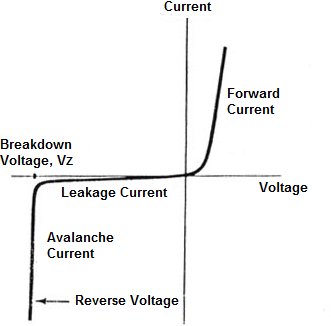
\includegraphics{Diode_Characteristics_Curve}
	\captionof{figure}{Diode Characteristic Curve}
\end{center}

% Equilibrium
\subsection{Equilibrium}

% -- Built-in Potential Barrier
\subsubsection{Built-in Potential Barrier}
\begin{empheq}[box={\mybluebox[5pt]}]{equation*}
V_{bi} = \frac{kT}{e}ln(\frac{N_aN_d}{n_i^2}) = V_Tln(\frac{N_aN_d}{n_i^2})
\end{empheq}

\begin{itemize}
\item e :=Charge of an Electron $(1.6x10^{-19} eV)$ \index{Charge of an Electron}
\item T := Temperature $(K)$ \index{Temperature}
\item k := Boltzmann's Constant $(86x10^{-6} \frac{eV}{k})$ \index{Boltzmann's Constant}
\item $n_i$ := Intrinsic Carrier Concentration $(\frac{\# of electrons}{cm^3})$ \index{Intrinsic Carrier Concentration}
\item $N_d$ := Donor Concentration $(cm^{-3})$ \index{Donor Concentration}
\item $N_a$ := Acceptor Concentration $(cm^{-3})$ \index{Acceptor Concentration}
\item $V_{bi}$ := Built-in Potential Barrier $(V)$ \index{Built-in Potential Barrier}
\item $V_T$ := Thermal Voltage at Room Temperature $(0.026 V)$ \index{Thermal Voltage}
\end{itemize}

% -- Thermal Voltage at Room Temperature
\subsubsection{Thermal Voltage at Room Temperature}
\begin{empheq}[box={\mybluebox[5pt]}]{equation*}
V_T = 0.026, (T=300k)
\end{empheq}

\cleardoublepage

% Forward-Biased
\subsection{Forward-Biased}

\cleardoublepage

% Reverse-Biased
\subsection{Reversed-Biased}

% -- Junction Capacitance
\subsubsection{Junction Capacitance}
\begin{empheq}[box={\mybluebox[5pt]}]{equation*}
C_j = C_{jo}(1+\frac{V_R}{V_{bi}})^{-1/2}
\end{empheq}

\begin{itemize}
\item $V_{bi}$ := Built-in Potential Barrier $(V)$ \index{Built-in Potential Barrier}
\item $V_R$ := Reverse-Bias Voltage $(V)$ \index{Reverse-Biase Voltage}
\item $C_j$ := Capacitance across a pn junction. $(pF)$ \index{Junction Capacitance}
\item $C_{jo}$ := Capacitance across a pn junction when there is no voltage applied. $(pF)$
\end{itemize}

% -- Reverse-Bias Saturation Current
\subsubsection{Reverse-Bias Saturation Current\index{Reverse-Bias Saturation Current}}
\begin{empheq}[box={\mybluebox[5pt]}]{equation*}
i_D = I_S[e^\frac{v_D}{V_T}-1]
\end{empheq}

\begin{itemize}
\item $i_D$ := Diode Current $(A)$ \index{Diode Current}
\item $v_D$ := Diode Voltage $(V)$ \index{Diode Voltage}
\item $V_T$ := Thermal Voltage at Room Temperature $(0.026 V)$ \index{Thermal Voltage}
\item $I_S$ := Reverse-Bias Saturation Current $(A)$ \index{Reverse-Bias Saturation Current}
\end{itemize}

\cleardoublepage
%-----------------------------------------------------------------------------------------------------------------------------------------------------------------------------
% --- --- --- --- --- --- --- ---  Bipolar Junction Transistors (BJT) --- --- --- --- --- --- --- --- 
\section{Bipolar Junction Transistors (BJT)}

% -- Current Relationships
\subsection{Current Relationships}

% formulas
\begin{empheq}[box={\mybluebox[5pt]}]{equation*}
i_C = I_Se^{v_{BE} / V_T}
\end{empheq}

\begin{empheq}[box={\mybluebox[5pt]}]{equation*}
i_C = \beta i_B
\end{empheq}

\begin{empheq}[box={\mybluebox[5pt]}]{equation*}
i_C = \alpha i_E
\end{empheq}

\begin{empheq}[box={\mybluebox[5pt]}]{equation*}
i_E = i_C + i_B
\end{empheq}

\begin{empheq}[box={\mybluebox[5pt]}]{equation*}
i_E = (1 + \beta )i_B
\end{empheq}

\begin{empheq}[box={\mybluebox[5pt]}]{equation*}
\alpha = \frac{\beta}{1 + \beta}
\end{empheq}

\begin{empheq}[box={\mybluebox[5pt]}]{equation*}
\beta = \frac{\alpha}{1 - \alpha}
\end{empheq}

% variables
\begin{itemize}
\item $i_B$ := Base Current $(A AC)$ \index{Base Current}
\item $i_C$ := Collector Current $(A AC)$ \index{Collector Current}
\item $i_E$ := Emitter Current $(A AC)$ \index{Emitter Current}
\item $i_S$ := Saturation Current $(A DC)$ \index{Saturation Current}
\item $\alpha$ := Common-Base Current Gain
\item $\beta$ := Common-Emitter Current Gain
\end{itemize}

\cleardoublepage

% Common Emitter Circuit
\subsection{Common-Emitter Circuit}

% npn DC Analysis
\subsubsection{npn DC Analysis}
\begin{center}
	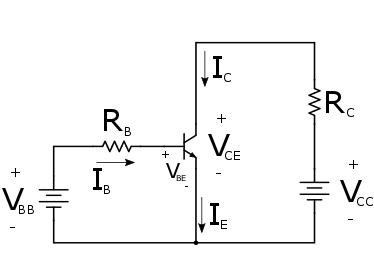
\includegraphics[width=100mm,scale=0.5]{Common-Emitter-Circuit-with-npn-BJT}
	\captionof{figure}{Common Emitter Circuit with npn BJT (DC Analysis)}
\end{center}

% formulas
\begin{empheq}[box={\mybluebox[5pt]}]{equation*}
I_B = \frac{V_{BB} - V_{BE}^{(on)}}{R_B}
\end{empheq}

\begin{empheq}[box={\mybluebox[5pt]}]{equation*}
V_{CC} = I_CR_C + V_{CE}
\end{empheq}

\begin{empheq}[box={\mybluebox[5pt]}]{equation*}
P_T = I_BV_{BE}^{(on)} + I_CV_{CE}
\end{empheq}

\begin{empheq}[box={\mybluebox[5pt]}]{equation*}
P_T \cong I_CV_{CE}
\end{empheq}

\begin{itemize}
\item $R_B$ := Base Resistance $(\Omega)$ \index{Base Resistance}
\item $R_C$ := Collector Resistance $(\Omega)$ \index{Collector Resistance}
\item $I_B$ := Base Current $(A DC)$ \index{Base Current}
\item $I_C$ := Collector Current $(A DC)$ \index{Collector Current}
\item $I_E$ := Emitter Current $(A DC)$ \index{Emitter Current}
\item $V_{BE}$ := Base-Emitter Voltage $(V)$ \index{Base-Emitter Voltage}
\item $V_{CE}$ := Collector-Emitter Voltage $(V)$ \index{Collector-Emitter Voltage}
\item $V_{BB}$ := Base Voltage $(V)$ \index{Base Voltage}
\item $V_{CC}$ := Collector Voltage $(V)$ \index{Collector Voltage}
\end{itemize}

\cleardoublepage

% pnp DC Analysis
\subsubsection{pnp DC Analysis}
\begin{center}
	
\end{center}
\cleardoublepage

% AC Analysis
\subsubsection{npn AC Analysis}
\begin{center}
	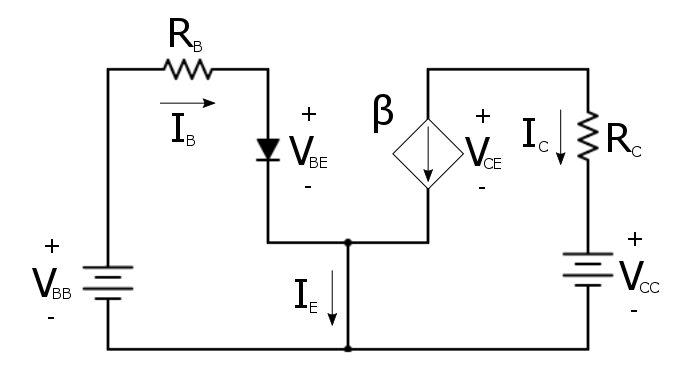
\includegraphics[width=100mm,scale=0.5]{Common-Emitter-Circuit-with-npn-BJT-AC-Analysis-1}
	\captionof{figure}{Common Emitter Circuit with npn BJT (AC Analysis)}
\end{center}

\begin{empheq}[box={\mybluebox[5pt]}]{equation*}
I_B = \frac{V_{BB} - V_{BE}^{(on)}}{R_B}
\end{empheq}

\begin{empheq}[box={\mybluebox[5pt]}]{equation*}
V_{CC} = I_CR_C + V_{CE}
\end{empheq}

\begin{empheq}[box={\mybluebox[5pt]}]{equation*}
P_T = I_BV_{BE}^{(on)} + I_CV_{CE}
\end{empheq}

\begin{empheq}[box={\mybluebox[5pt]}]{equation*}
P_T \cong I_CV_{CE}
\end{empheq}

\begin{itemize}
\item $R_B$ := Base Resistance $(\Omega)$ \index{Base Resistance}
\item $R_C$ := Collector Resistance $(\Omega)$ \index{Collector Resistance}
\item $i_B$ := Base Current $(A AC)$ \index{Base Current}
\item $i_C$ := Collector Current $(A AC)$ \index{Collector Current}
\item $i_E$ := Emitter Current $(A AC)$ \index{Emitter Current}
\item $V_{BE}$ := Base-Emitter Voltage $(V)$ \index{Base-Emitter Voltage}
\item $V_{CE}$ := Collector-Emitter Voltage $(V)$ \index{Collector-Emitter Voltage}
\item $V_{BB}$ := Base Voltage $(V)$ \index{Base Voltage}
\item $V_{CC}$ := Collector Voltage $(V)$ \index{Collector Voltage}
\end{itemize}

\cleardoublepage
%-----------------------------------------------------------------------------------------------------------------------------------------------------------------------------
% --- --- --- --- --- --- --- ---  Metal Oxide Semiconductor - Field Effect Transistors (MOSFET) --- --- --- --- --- --- --- --- 
\section{Metal Oxide Semiconductor - Field Effect Transistors (MOSFET)}
\cleardoublepage
%-----------------------------------------------------------------------------------------------------------------------------------------------------------------------------
% Appendices, Indexes, and Glossaries
\pagenumbering{roman}
\setcounter{page}{1}

\addcontentsline{toc}{section}{Variables}
\printglossary[type=\acronymtype,nonumberlist,title={Variables}]
\clearpage
\addcontentsline{toc}{section}{Glossary}
\glsaddall
\printglossary[nonumberlist]
\clearpage
%-----------------------------------------------------------------------------------------------------------------------------------------------------------------------------
\printindex
\clearpage
%-----------------------------------------------------------------------------------------------------------------------------------------------------------------------------
% Bibliography
\addcontentsline{toc}{section}{Refrences}
\bibliographystyle{plain}
\bibliography{transistorbib}
%-----------------------------------------------------------------------------------------------------------------------------------------------------------------------------
\end{document}
%-----------------------------------------------------------------------------------------------------------------------------------------------------------------------------